\documentclass[letter, 10pt]{article}
% Change "article" to "report" to get rid of page number on title page
\usepackage{amsmath,amsfonts,amsthm,amssymb}
\usepackage{setspace}
\usepackage{graphicx,float,wrapfig}
%\usepackage{parskip}
\usepackage{enumerate}

\usepackage{fourier}
\usepackage[T1]{fontenc}
\usepackage[protrusion=true,expansion=true]{microtype}

% In case you need to adjust margins:
\topmargin=-0.45in      %
\evensidemargin=0in     %
\oddsidemargin=0in      %
\textwidth=6.5in        %
\textheight=9.0in       %
\headsep=0.25in         %
\parindent=0in

\usepackage[nodayofweek]{datetime} \usdate
% Pdf metadata
\pdfinfo{  /Author (Blake Riley)
           /Title (Econ 533 Handout 4)
           /Keywords ()
           /ModDate (D:\pdfdate)}

\newtheoremstyle{basic}% name
   {5pt}% Space above
   {5pt}% Space below
   {\itshape \leftskip=1em}% Body font
   {-1em}% Indent amount
   {\bfseries}% Theorem head font
   {:}% Punctuation after theorem head
   { }% Space after theorem head
   {}% Theorem head spec (can be left empty, meaning `normal')
\theoremstyle{basic}
\newtheorem{exercise}{Exercise}[section]
\newtheorem{definition}{Definition}[section]
\newtheorem{theorem}{Theorem}[section]
\newtheorem{lemma}[theorem]{Lemma}


%%%%%%%%%%%%%%%%%%%%%%%%%%%%%%%%%%%%%%%%%%%%%%%%%%%%%%%%%%%%

% Custom commands

\newcommand{\R}{\mathbb{R}}
\newcommand{\N}{\mathbb{N}}
\newcommand{\E}{\operatorname{E}}
\renewcommand{\P}{\operatorname{Pr}}
\newcommand{\Var}{\operatorname{Var}}
\newcommand{\Cov}{\operatorname{Cov}}
\newcommand{\cond}{\,|\,}
\newcommand{\bigcond}{\;\big|\;}
\newcommand{\argmax}{\mathop{\operatorname{arg\,max}}}
\newcommand{\noti}{{{\scriptscriptstyle-}\!i}}
\newcommand{\notj}{{{\scriptscriptstyle-}\!j}}
\newcommand{\notij}{{{\scriptscriptstyle-}\!\{i,j\}}}
\newcommand{\I}{\mathbb{I}}

%%%%%%%%%%%%%%%%%%%%%%%%%%%%%%%%%%%%%%%%%%%%%%%%%%%%%%%%%%%%%
%%%%%%%%%% The main document content
%%%%%%%%%%%%%%%%%%%%%%%%%%%%%%%%%%%%%%%%%%%%%%%%%%%%%%%%%%%%%

\begin{document}
\begin{spacing}{1.0}

\noindent
\textbf{Handout 4} \\
Econ 533 \\
February 26, 2015 \\
TA: Blake Riley \\

\section{Social Choice Theory}

Social choice theory deals with the aggregation of
individual preferences over some number of
alternatives. The arising aggregated preferences then
reflect some sort of social preferences, and like
individual preferences, we want these to satisfy certain
conditions. For example, we may want unanimous agreement
on the best option to be maintained in the social ranking
by placing this option on top.

\subsection{Notation}

We consider the following $\mathcal{E} = \{X,
\succeq_i\}_{i=1}^n$ as representing a social group or
economy, where $n$ is the number of agents in the
economy. We consider identical sets of alternatives $X$
for each individual, and heterogeneous, rational
(complete and transitive) preference relations. We denote
with $R$ the set of all possible rational (weak)
preferences relations on $X$ and $P$ as the set of all
strict rational preferences. A typical element of $R
\times R \times \ldots \times R = R^n$ is $(\succeq_1,
\ldots, \succeq_n)$, which will be called a preference
profile. If $X$ is finite, then each profile is a
collection of $n$ rankings of the alternatives.

\section{Social Welfare Functions}

\begin{definition}
  A \textbf{social welfare function} is a rule $F: A\to
  R$ (with $A= R^n$ or $P^n$) that assigns a rational
  preferences relation $F(\succeq_1, \ldots, \succeq_n)
  \in R$, interpreted as the social preference relation,
  to any profile of individual rational preferences in $A$.
\end{definition}

\begin{definition}
  A social welfare function $F:A\to R$ is
  \textbf{Pareto-efficient} or
  \textbf{Paretian} if, for all alternatives
  $x,y \in X$ and all preference profiles
  $\succeq=(\succeq_1, \ldots, \succeq_n)\in A$, we have \[\forall
  i\in n, \, x \succ_i y \implies x \, F(\succeq) \, y\]
\end{definition}

\begin{definition}
  A social welfare function $F:A\to R$ satisfies
  \textbf{independence of irrelevant alternatives (IIA)}  if for
  all $x,y \in X$ and for all pairs of profiles
  $\succeq , \succeq'\, \in A$ with the property \[x\succeq_i y
  \iff x\succeq'_i y \quad\text{ and }\quad y \succeq_i x \iff y
  \succeq'_i x\] we have \[x\, F(\succeq) \, y \iff x
  \,F(\succeq')\, y \quad\text{ and }\quad y\, F(\succeq) \, x \iff y
  \,F(\succeq')\, x\]
\end{definition}

\begin{definition}
  A social welfare function $F: A\to R$ is
  \textbf{dictatorial} if there is an agent $h\in n$ such
  that for all $x,y \in X$ and for all $\succeq \,\in A$, we
  have $x \succeq_h \implies x\, F(\succeq) \, y$.
\end{definition}

\section{Social Choice Functions}

Social preferences aren't that useful unless they are
used to make some sort of social choice. Given that, we
can represent the process of making a choice from a set
of options based on a preference profile as a single function.

\begin{definition}
  A \textbf{social choice function} is a rule $f: A\to X$
  (with $A = R^I$ or $p^I$) that assigns a chosen element
  $f(\succeq_1, \ldots, \succeq_I) \in X$ to every profile
  of individual rational preference relations in $A$.
\end{definition}

At the moment, we are assuming a single-valued function,
but this can readily be extended to a correspondence following Maskin.

\begin{definition}
  A social choice function $f: A \to X$ is \textbf{weakly
    Pareto efficient} is, for all preference profiles
  $\succeq\, \in A$, the choice $f(\succeq) \in X$ is a
  weak Pareto optimum, i.e. for all $x,y\in X$ such that
  $x \succ_i y$ for all $i\in n$, then $y \not = f(\succeq)$.
\end{definition}

\begin{definition}
  The alternative $x\in X$ \textbf{maintains its
    position} from $\succeq\,\in R^n$ to $\succeq' \,\in
  R^n$ if $x \succeq_i y \implies x \succeq' y$ for all
  $i\in n$ and $y \in X$. Equivalently, the lower contour
  sets of $x$ in the preferences of the first profile are
  subsets of the lower contour sets of the corresponding
  preferences in the second profile.
\end{definition}

\begin{definition}
  A social choice function $f: A \to X$ is
  \textbf{monotonic} if for all profiles $\succeq,
  \succeq'\,\in A$ where $x = f(\succeq)$ maintains its
  position from $\succeq$ to $\succeq'$, we have
  $f(\succeq')=x$ again.
\end{definition}

\begin{definition}
  A social choice function is \textbf{dictatorial} if
  there exists an agent $h\in n$ such that for all
  profiles $\succeq \,\in A$, we have $f(\succeq) =
  \{x\;|\; \forall y\in X, x\succeq_h y\}$,
  i.e. $f(\succeq)$ is a maximal element for $h$ over $X$.
\end{definition}

\begin{definition}
  A social choice function is \textbf{strategy-proof} if
  for all $i\in n$, preferences profile $\succeq\,\in A$,
  and alternate preference $\succeq'_i \in R$, we have
  $f(\succeq_i, \succeq_{-i}) \succ_i f(\succeq'_i, \succeq_{-i})$.
\end{definition}

\section{Impossibility Results}

\begin{theorem}
  (Arrow 1950) Suppose $|X| \geq 3$ and $A = R^n$ or
  $P^n$. Then every social welfare function $F:A\to R$
  that is Pareto-efficient and satisfies IIA is dictatorial.
\end{theorem}

\begin{theorem}
  (Muller and Satterthwaite 1977) Suppose $|X| \geq 3$
  and $A = R^n$ or $P^n$. Then every social choice
  function $f:A \to X$ that is weakly Pareto-efficient
  and monotonic is dictatorial.
\end{theorem}

\begin{theorem}
  (Gibbard 1973, Satterthwaite 1977) If  $|X| \geq 3$ and
  the social choice function $f: A \to X$ is onto (surjective) and
  strategy-proof, then $f$ is dictatorial.
\end{theorem}

\section{Mechanism Design}

With social choice theory, we looked at how to aggregate preferences
assuming these were observable. Gibbard-Satterthwaite points us toward the
direction of imperfectly observable preferences that must be revealed by
the individuals before they can be aggregated.

\hspace{1em}
We again consider a set of agents $n$ which will make a collective choice
form a set of alternatives $X$. Utility functions $u_i(x, \theta_i)$ are
commonly known, but are determined by a pivately known random variable
$\theta_i \in \Theta_i$ which is the agent's type. Typically there is a
commonly known prior $\phi(\cdot)$ representing a density over $\theta \in
\Theta_1 \times \ldots \times \Theta_n$. Since the utility functions
themselves are common knowledge in this context, all uncertainty handled is
through the type. Types can also encode the beliefs of an agent. Our new
formulation of a social choice function is a straightforward extension
based on this.

\begin{definition}
  A \textbf{social choice function} is a rule $f:
  \Theta_1 \times \ldots \times \Theta_n \to X$ that
  assigns a chosen element $f(\theta) \in X$ for each
  profile of individual preferences derived from the
  vector of types $\theta$.
\end{definition}

Some properties are also simple extensions:

\begin{definition}
  The social choice function $f: \Theta \to X$ is
  \textbf{ex-post efficient} if for all $\theta \in
  \Theta$ there does not exist an $x \in X$ such that
  $u_i(x, \theta_i) \geq u_i(f(\theta), \theta_i)$ for
  all $i$ and $u_i(x, \theta_i) > u(f(\theta), \theta_i)$
  for some $i$.
\end{definition}

\section{Mechanisms and Implementation}

Since agents' types are private information, they must communicate this
information to the rest of the group or a central body. We could have any
theory about how agents choose the messages they will send, but we
typically assume messages will be chosen strategically. Once the messages
are collected, an outcome will be chosen by the group. Together, the
possible messages and the mapping from messages to outcomes define a
mechanism.

\begin{definition}
  A \textbf{mechanism} $\xi = \{(M_1, \ldots, M_n),
  g(\cdot)\}$ is a collection of $n$ message sets (or
  strategy sets) and an outcome function $g: M_1 \times
  \ldots \times M_n \to X$.
\end{definition}

Mechanisms can be considered as procedures for how a
collective decision is actually made, including a specification of
strategy sets. We can now compare what outcomes are
realized in equilibrium through a mechanism with the
outcomes we ``want'' to see happen, as represented by a
social choice function. If an outcome function $g$ and
a social choice function $f$ coincide on some restriction
of their domain, then we say $g$ implements $f$. The
particular restriction depends on the equilibrium concept used.

\begin{definition}
  The mechanism $\xi = \{(M_1, \ldots, M_n),
  g(\cdot)\}$ \textbf{implements} a social choice function $f$ if
  there is an equilibrium strategy profile
  $(m_1^*(\cdot), \ldots, m_n^*(\cdot))$ of the game
  induced by $\xi$ such that $\forall \theta \in \Theta$,
  \[g(m_1^*(\theta_1), \ldots, m_n^*(\theta_n)) =
  f(\theta_1, \ldots, \theta_n)\]
\end{definition}

The term equilibrium here is still vague and we will extend this definition
to talk about implementation in various contexts. The mechanism itself
might have multiple equilibria. If the outcome of one equilibrium coincides
with the scf, then the scf is \textit{partially} implemented. If the
outcomes of all equilibria coincide with the scf, then the scf is
\textit{fully} implemented.  Figure \ref{reiterdiagram} depicts the generic
implementation problem.


\begin{figure}[ht!]
  \centering
  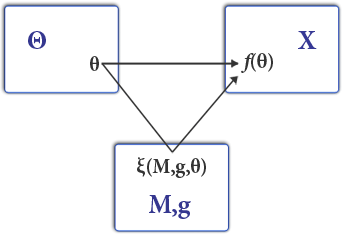
\includegraphics[width=.45\columnwidth]{reiterdiagram}
    \caption{Reiter diagram of a
  mechanism $\xi$ implementing $f$}
\label{reiterdiagram}
\end{figure}

Due to the revelation principle, we can usually think of
the message space as the type space, and most mechanisms
we'll look at are direct revelation mechanisms. This also
leads us to a notion of incentive compatibility.

\begin{definition}
  A \textbf{direct revelation mechanism} for $f$ is a mechanism
  in which $M_i = \Theta_i$ for all $i$ and $g(\theta) =
  f(\theta)$ for all $\theta \in \Theta_1 \times \ldots
  \times \Theta_I$.
\end{definition}

\begin{definition}
  The social choice function $f$ is \textbf{truthfully
    implementable} if the direct revelation mechanism has
  an equilibrium $(m_1^*(\cdot), \ldots, m_n^*(\cdot))$
  in which $m_i^*(\theta_i) = \theta_i$ for all $i$ and
  $\theta$, i.e. each agent telling the truth is an
  equilibrium of the induced game. Alternatively, such a
  mechanism is \textbf{incentive compatible}.
\end{definition}

\section{Dominant Strategy Implementation}
\label{sec:domin-strat-impl}

\begin{definition}
  A mechanism $\xi = \{(M_1, \ldots, M_n),
  g(\cdot)\}$ is a \textbf{dominant-strategy
    implementation} of a social choice function $f$ if
  there is a dominant strategy equilibrium profile
  $(m_1^*(\cdot), \ldots, m_I^*(\cdot))$ of the game
  induced by $\xi$ such that $\forall \theta \in \Theta$,
  $g(m_1^*(\theta_1), \ldots, m_I^*(\theta_I)) =
  f(\theta_1, \ldots, \theta_I)$.
\end{definition}

Here we start with some scf $f$ and ask whether a mechanism exists such
that the outcome from agents playing a dominant strategy matches the scf
for all realization of types. If this was the case, then we would have a
very robust way of implementing the scf, since we can be confident about
what agents will want to do, regardless of what other agents do or what their types are.

\hspace{1em}
Incentive compatibility in this context is also a simple
extension.
\begin{definition}\label{IC}
  The scf $f(\cdot)$ is \textbf{truthfully implementable in dominant
  strategies} or \textbf{strategy-proof} if for all $i$ and $\theta_i$, \[u_i(f(\theta),\theta_i, \theta_{-i})
  \geq u_i(f(\hat{\theta}_i, \theta_{-i}),
  \hat{\theta}_i, \theta_{-i})\] for all $\hat{\theta}_i$
  and $\theta_{-i}$.
\end{definition}

Now we have the powerful, if nearly trivial,
revelation principle for dominant strategy implementation:
\begin{theorem}
  Suppose there exists a mechanism $\xi$ that implements
  $f$ in dominant strategies. Then $f$ is truthfully
  implementable in dominant strategies.
\end{theorem}

Checking whether an arbitrary scf can be implemented in dominant strategies
seems like a monumental task; imagine trying to search over all possible
procedures for making a choice. By this theorem though, we know if there is
such a mechanism, there is also a direct revelation mechanism where
agents report their types honestly. Hence, checking implementability
reduces to checking the inequalities in Definition \ref{IC}. This
holds for many other equilibrium concepts, which justifies looking only at
revelation mechanisms. Of course, this assumes it's practical for agents to
fully communicate their types, which could potentially include a full set
of beliefs, beliefs about beliefs, etc, without cost, so we might be
trading one intractability for another.

\section{Nash Implementation}
\label{sec:nash-implementation}

Maskin focuses on general preferences and social choice correspondences,
which leads to the following definition:

\begin{definition}
  A mechanism $\{(S_i, \ldots, S_I), g(\cdot)\}$ with
  $g:\prod S_i \to X$ implements the social choice
  rule $f: \prod R_i \twoheadrightarrow X$ in Nash
  equilibrium if
  \begin{enumerate}
  \item $\forall x \in f(\succeq), \, \exists (s_1, \ldots,
    s_I)$ such that $x = g(s_1, \ldots, s_I)$ and $x \succeq_i g(s'_i, s_{-i})$ for all $i$ and all $s'_i$.
  \item If $(s_1, \ldots, s_I)$ is a Nash equilibrium,
    then $g(s) \in f(\succeq)$.
  \end{enumerate}
\end{definition}

The first part extends our implementation to
correspondences, while the second requires that all Nash
equilibria result in outcomes in the social choice
rule. Then, Maskin gives us the following result:

\begin{theorem}
  If $f: R^n \twoheadrightarrow X$ is implementable in
  Nash equilibrium, then $f$ is monotonic.
\end{theorem}

This provides an easy first check to see whether a scr is
Nash-implementable. However, the converse is not
true. We'll need another condition:

\begin{definition}
  A scr $f: R^n \twoheadrightarrow X$ satisfies
  \textbf{no veto power (NVP)} if for all preference
  profiles $\succeq$ and all $x\in X$, then for all agents
  $i$ we have \[\forall j \neq i, \forall y\in X, \, x \succeq_j
  y \implies x\in f(\succeq)\]
\end{definition}

\begin{theorem}
  With at least three players, if $f$ is monotonic and
  satisfies NVP, then $f$ is Nash-implementable.
\end{theorem}

\newpage
\section{Exercises}
\label{sec:exercises}

\begin{exercise}[p. 57 of \textit{Toolbox for Economic Design}]
  Assume a social choice function $f: \Theta \to X$ is
  dominant-strategy incentive compatible. Let $\bar{f}: \bar{\Theta} \to
  X$, where $\bar{\Theta} \subset \Theta$, be the restriction of $f$ to
  $\bar{\Theta}$, i.e. $\theta \in \bar{\Theta} \implies \bar{f}(\theta) =
  f(\theta)$. Is $\bar{f}$ also dominant-strategy incentive compatible?
\end{exercise}

\begin{exercise}[p. 56 of \textit{Toolbox for Economic Design}]
  Imagine a society that consists of a single couple, Link and Zelda. The
  couple is trying to decide whether to paint their castle black, white, or
  silver. Zelda has one type $\theta_Z$. Her ranking is
  white~$\succ$~silver~$\succ$~black. Link, on the other hand, has two
  possible types: $\theta_L$ and $\bar{\theta}_L$. When his type is
  $\theta_L$, his ranking is black~$\succ$~silver~$\succ$~white. When he is
  type $\bar{\theta}_L$, his ranking is
  silver~$\succ$~white~$\succ$~black.
  \begin{enumerate}
  \item Suppose we wish to implement the following social choice function:
    $f(\theta_Z, \theta_L) =$ silver and $f(\theta_Z, \bar{\theta}_L) =$
    white. Will Link choose to truthfully reveal his type?
  \item What if the desired social choice function is
    $f(\theta_Z, \theta_L) =$ black and $f(\theta_Z,
    \bar{\theta}_L) =$ white?
  \item What about  $f(\theta_Z, \theta_L) =$ silver and $f(\theta_Z,
  \bar{\theta}_L) =$ silver?
  \end{enumerate}
\end{exercise}

\begin{exercise}[Sprumont 1991]
  One useful restriction of preferences is \emph{single-peakedness}. If the
  set of options $X$ is single-dimensional and ordered, then a preference
  ordering $\succ$ on $X$ is single-peaked iff there is a maximum $x^*$ of
  $\succ$ and $x^* < x < y$ or $y < x < x^* \implies x \succ y$.

  \hspace{1em}
  Consider a partnership of $n$ individuals who will invest in a project,
  with the benefits shared in proportion to each partner's investment. The
  project has a fixed cost of $1$. The partners have single-peaked
  preferences over the amount they want to invest, with a peaks $x_i^* \in
  [0,1]$. Because the sum of the peak amount of all partners may not be
  equal to the cost of the project, some partners may be forced to invest
  more or less than their ideal amounts. In this context, efficiency means
  that if the sum of ideal investments is less than the cost, everyone must
  invest at least their ideal amount, and vice versa.

  \hspace{1em}
  In addition to strategy-proofness and efficiency, let's consider two
  other desirable properties of social choice functions. First, an scf is
  \emph{anonymous} if $f(\theta)=f(\pi(\theta))$ for all permutations $\pi$
  of the vector. Second, an scf is \emph{envy-free} if for all $i,j$,
  $f_i(\theta) \succeq_i f_j(\theta)$, i.e. the proportion allocated to $i$
  is preferred by $i$ to all other agents' allocations.

  \hspace{1em}
  Check whether the following are strategy-proof,
  efficient, anonymous, and/or envy-free:
  \begin{enumerate}
  \item The egalitarian rule $f_i^e(\theta) = 1/n$.
  \item The proportional rule $f_i^p(\theta) = x_i^*/\sum x_j^*$.
  \item The priority rule $f_1^q(\theta) = x_1^*$ and
    $f_i^q(\theta) = \min\{x_i^*, 1-\sum_{j<i} x_j^*\}$
    when $\sum x_i^* \geq 1$, and alternately $f_j^q(\theta) = x_j^*$
    for $j < n$ and $f_n^q(\theta) = 1 - \sum_{j=1}^{n-1}
    x_j^*$ when $\sum x^i < 1$.
  \item The priority rule as defined above, but with a random order.
  \item The uniform rule defined by the iterative process (for the case of
    $\sum x_i^* > 1$):
    \begin{enumerate}
    \item Start with all partners active and the full cost outstanding.
    \item Divide the outstanding cost equally among the active partners.
    \item If any active partner has an ideal below the equal
      share, set their share equal to their ideal and
      subtract this from the outstanding cost. These
      partners are now inactive.
    \item Repeat the previous two steps among the active
      partners until each has an ideal amount no less
      than the equal share of the outstanding cost.
    \end{enumerate}

  \end{enumerate}

\end{exercise}


%%%%%%%%%%%%%%%
\end{spacing}
\end{document}
%%%%% FIN %%%%%
%%%%%%%%%%%%%%%